\pagebreak
\section{Logarithmus}\label{sec:E-Funktion/Logarithmus}
Betrachtet man folgendes, könnte auffallen, dass es einen Beziehung zwischen $n$,$b$ und $r$ geben könnte.  
\begin{align*}
	b^n=r
\end{align*}
\paragraph{Die Potenz} beschreibt zunächst den Weg, wie man zu $r$ kommt. Dies erfolgt durch das Potenzieren der Basis $b$ mit dem Exponenten $n$
\paragraph{Die Wurzel} beschreibt die Beziehung zwischen $r$ und $n$ und ergibt abschließend $b$
\paragraph{Der Logarithmus} beschreibt die Beziehung zwischen der Basis $b$ und dem Ergebnis $r$.
\begin{figure}[h]
	\centering
	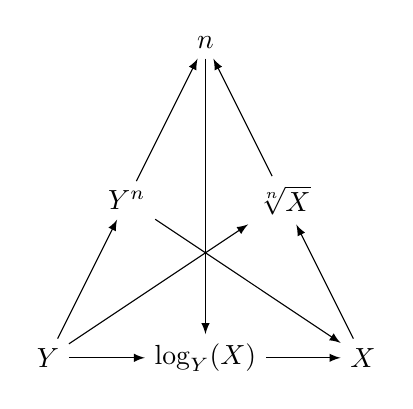
\begin{tikzpicture}[>=latex,font=\sffamily]
  % Knoten
  \node (b) at (0,0) {$Y$};
  \node (bn) at (1,2) {$Y^n$};
  \node (E) at (4,0) {$X$};
  \node (n) at (2,4) {$n$};
  \node (nrootE) at (3,2) {$\sqrt[n]{X}$};
  \node (logbE) at (2,0) {$\log_Y(X)$};

  % Pfeile
  \draw[->] (b) -- (bn) node[midway,left] {};
  \draw[->] (bn) -- (n) node[midway,left] {};
  \draw[->] (E) -- (nrootE) node[midway,right] {};
  \draw[->] (nrootE) -- (n) node[midway,right] {};
  \draw[->] (b) -- (logbE) node[midway,below] {};
  \draw[->] (logbE) -- (E) node[midway,below] {};

  % Diagonale Linien
  \draw[->] (b) -- (nrootE);
  \draw[->] (bn) -- (E);
  \draw[->] (n) -- (logbE);
  % Beschriftungen
\end{tikzpicture}
	\caption{Auswirkung von $a$ auf den Graphen}
\end{figure}
\subsubsection{Entstehung}\label{sec:E-Funktion/Logarithmus/Entstehung}
Dem Logarithmus liegt die Mercator-Reihe zugrunde und ist lediglich eine Approximation... 
%TODO Hier fehlt eine Erklärung
\subsubsection{Bedeutung}\label{sec:E-Funktion/Logarithmus/Bedeutung}
Durch die Eigenschaften des Logarithmus kann man sagen, dass dieser das Verhältnis zwischen 
\subsubsection{Anwendung}\label{sec:E-Funktion/Logarithmus/Anwendung}
\subsection{Logarithmus naturalis} Der Logarithmus naturalis ist der Logarithmus zu der Basis $e$ und wird als verkürzte Schreibweise für $log_e(n)$ genutzt. 
\subsection{Logaritmus Gesetzt}
\pagebreak
\section{Ableitung des Logarithmus Naturalis}
Genauso wie andere Funktion besitzt der $ln$ eine Ableitung. Die Besonderheit ist hierbei allerdings, dass die Ableitung des $ln(x)$ immer $\frac{1}{x}$ ist. Als Erklärung kann man sich folgendes Anschauen:
\begin{align*}
	x&=e^{ln(x)}\tag{Ableiten auf beiden Seiten}\\
	1&=(ln(x))'\cdot e^{ln(x)}\tag{Beide Seiten vereinfachen}\\
	1&=(ln(x))'\cdot x\tag{Durch $x$ dividieren}\\
	\frac{1}{x}&=(ln(x))'\\	
\end{align*}
\pagebreak
\section{Verschiebung \& Streckung des $ln(x)$}
Genauso wie die $e$-Funktion lässt sich der $ln$ ebenfalls im Koordinatensystem durch verschiedene Parameter modelieren. Hierbei kommt die Normalform des $ln(x)$ zum Einsatz.
\[f(x)=a\cdot ln(b\cdot(x-c))+d\]
\subsubsection{$a$ - Streck- oder Stauchungsfaktor}
Der Streck- oder Stauchungsfaktor sorgt für eine Streckung oder Stauchung an der $Y$-Achse. Der Grund hierfür ist, dass zunächst die Werte auf $Y$-Achse mit dem $ln$ berechnet werden und anschließend mit $a$ multipliziert werden. Somit bleibt ebenfalls die Nullstelle erhalten, da sich beim Multiplizieren mit Null (wenn man in $ln(x)$ die Zahl $1$ einsetzt) immer Null ergibt. 
\begin{figure}[h]
\centering
	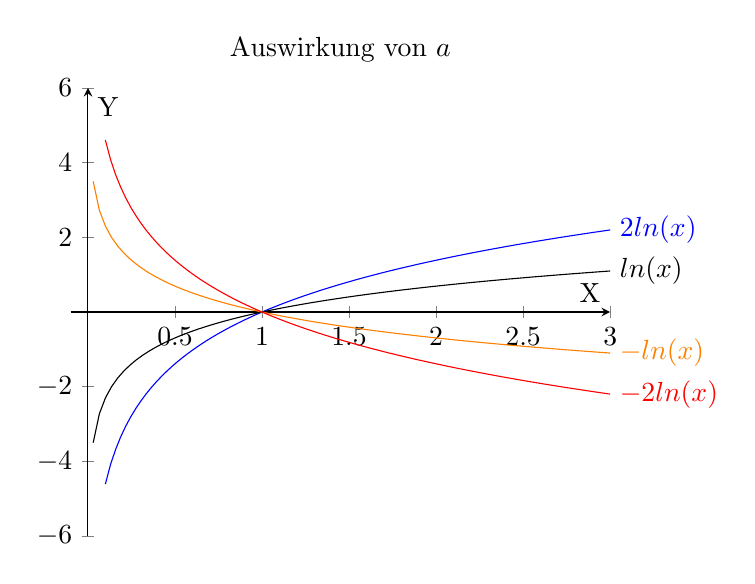
\begin{tikzpicture}
		\begin{axis}[
		title={Auswirkung von $a$},
		axis lines=middle,
		clip=false,
		xlabel={X},
		ylabel={Y},
		xmin=-0.1,
		xmax=3,
		ymin=-6,
		ymax=6
		]
		\addplot[domain=0.1:3,blue, samples=100]{2*ln(x)} node[right,pos=1]{$2ln(x)$};
		\addplot[domain=-0.5:3,black,samples=100]{ln(x)}node[right,pos=1]{$ln(x)$};
		\addplot[domain=-0.5:3,orange,samples=100]{-ln(x)}node[right,pos=1]{$-ln(x)$};
		\addplot[domain=0.1:3,red,samples=100]{-2*ln(x)}node[right,pos=1]{$-2ln(x)$};
		\end{axis}
	\end{tikzpicture}
	\caption{Auswirkung von $a$ auf den Graphen}
\end{figure}
\pagebreak
\subsubsection{$b$ - Streck- oder Stauchfaktor}
Der Koeffizent $b$ ist ebenfalls ein Stauchungs- oder Streckfaktor im Bezug auf den Graphen. Allerdings streckt dieser den Graphen auf der $X$-Achse, indem er die $x$-Werte bevor sie durch den $ln$ nacher die $Y-Wert$ ergeben, multipliziert. Das Bedeutet, dass die $Y$- Werte, die eigentlich an einem anderen Wertepaar erst erreicht werden mit einem davorliegenden $x$ erreicht werden. Außerdem spiegelt man mit diesem Faktor den Graphen an der $Y$-Achse.  
\begin{paracol}{2}
	\begin{flushleft}
	\begin{beispiel}
	\begin{align*}
		f(x)=ln(x)\\
		f(3)=ln(3)\\
		f(3)=1.09\\
	\end{align*}
\end{beispiel}
	\end{flushleft}	
\switchcolumn
	\begin{flushright}
		\begin{beispiel}
	\begin{align*}
		f(x)=ln(2x)\\
		f(3)=ln(2\cdot3)\\
		f(3)=1.79\\
	\end{align*}
\end{beispiel}
	\end{flushright}
\end{paracol}
\begin{figure}[h]
\centering
	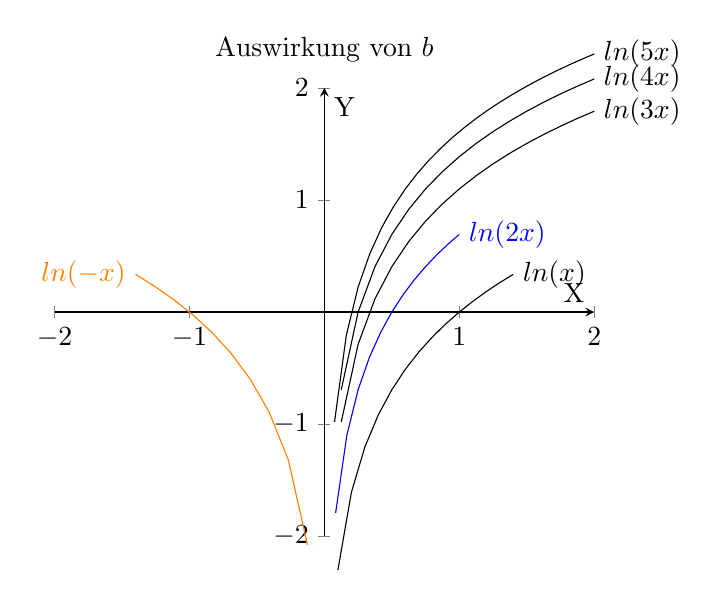
\begin{tikzpicture}
		\begin{axis}[
		title={Auswirkung von $b$},
		axis lines=middle,
		clip=false,
		xlabel={X},
		ylabel={Y},
		xmin=-2,
		xmax=2,
		ymin=-2,
		ymax=2
		]
		\addplot[domain=-1:1,blue]{ln(2*x)} node[right,pos=1]{$ln(2x)$};
		\addplot[domain=-1:1.4,black]{ln(x)}node[right,pos=1]{$ln(x)$};
		\addplot[domain=-1.4:2,orange]{ln(-x)}node[left,pos=0]{$ln(-x)$};
		\addplot[domain=-1:2,black]{ln(3*x)}node[right,pos=1]{$ln(3x)$};
		\addplot[domain=-1:2,black]{ln(4*x)}node[right,pos=1]{$ln(4x)$};
		\addplot[domain=-0.1:2,black]{ln(5*x)}node[right,pos=1]{$ln(5x)$};
		\end{axis}
	\end{tikzpicture}
	\caption{Auswirkung von $b$ auf den Graphen}
\end{figure}
\pagebreak
\subsubsection{$c$-Verschiebung auf $X$-Achse} Mit $c$ lässt sich der Graph auf der $Y$-Achse verschieben. Ist $c<0$ verschiebt sich hierbei der Graph nach rechts. Ist $x>0$ verschiebt er sich nach links.

\begin{figure}[h]
\centering
	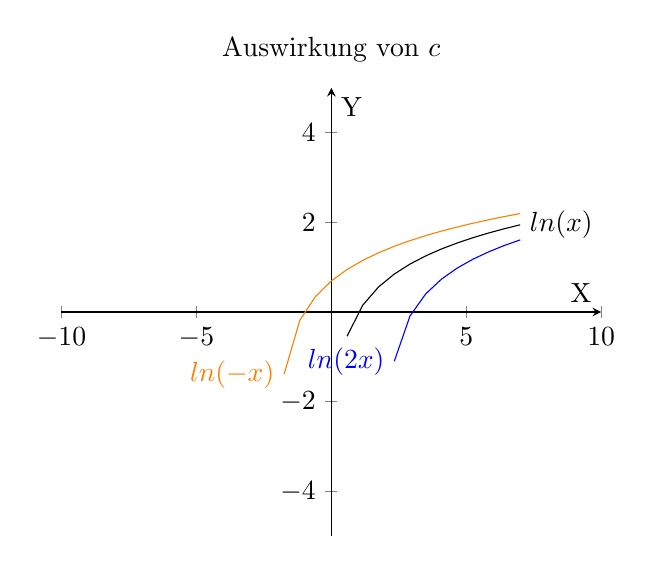
\begin{tikzpicture}
		\begin{axis}[
		title={Auswirkung von $c$},
		axis lines=middle,
		clip=false,
		xlabel={X},
		ylabel={Y},
		xmin=-10,
		xmax=10,
		ymin=-5,
		ymax=5
		]
		\addplot[domain=-7:7,blue]{ln(x-2)} node[left,pos=0]{$ln(2x)$};
		\addplot[domain=-7:7,black]{ln(x)}node[right,pos=1]{$ln(x)$};
		\addplot[domain=-7:7,orange]{ln(x+2)}node[left,pos=0]{$ln(-x)$};
		\end{axis}
	\end{tikzpicture}
	\caption{Auswirkung von $c$ auf den Graphen}
\end{figure}
\pagebreak
\subsubsection{$b$ - Y-Achsenverschiebung}
Der Summand $b$ sorgt für eine $Y$-Achsenverschiebung, da zu den $X$-Werten jeweils ein gewisser Wert addiert oder subtrahiert wird.
\begin{figure}[h]
\centering
	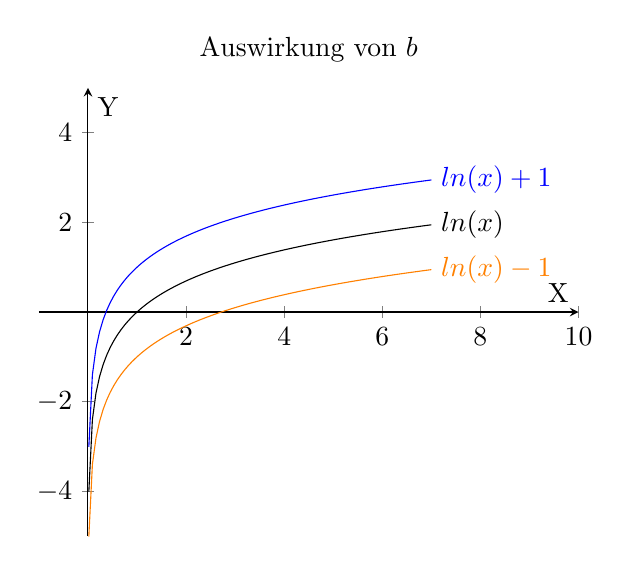
\begin{tikzpicture}
		\begin{axis}[
		title={Auswirkung von $b$},
		axis lines=middle,
		clip=false,
		xlabel={X},
		ylabel={Y},
		xmin=-1,
		xmax=10,
		ymin=-5,
		ymax=5
		]
		\addplot[domain=-0.2:7,blue, samples=100]{ln(x)+1} node[right,pos=1]{$ln(x)+1$};
		\addplot[domain=-0.2:7,black, samples=100]{ln(x)}node[right,pos=1]{$ln(x)$};
		\addplot[domain=-0.2:7,orange, samples=100]{ln(x)-1}node[right,pos=1]{$ln(x)-1$};
		\end{axis}
	\end{tikzpicture}
	\caption{Auswirkung von $b$ auf den Graphen}
\end{figure}


